\section{Controller hardware}
%The controller is build around an \amega that receives data from the DB-25 connector on the cranes front panel. Some additional hardware is also added to the controller, 2 switches, 2 LED's with resistors, a 4x16 LCD display, a joystick with 2 \SI{4.7}{\kilo\ohm} and a button build in.

The controller is build in a plastic case with a DB-25 connector and a hole for uploading new software on the board. The controller is build around an \amega that receives data from the DB-25 connector on the cranes front panel. On the lid the joystick, two switches and two LED's are mounted provide the manual input to the system. An OLED screen is also mounted on the lid to make it possible to provide the user various data while controlling the crane. The controller is shown in figure \ref{fig:pic_of_controller}.

\begin{figure}[H]
    \centering
    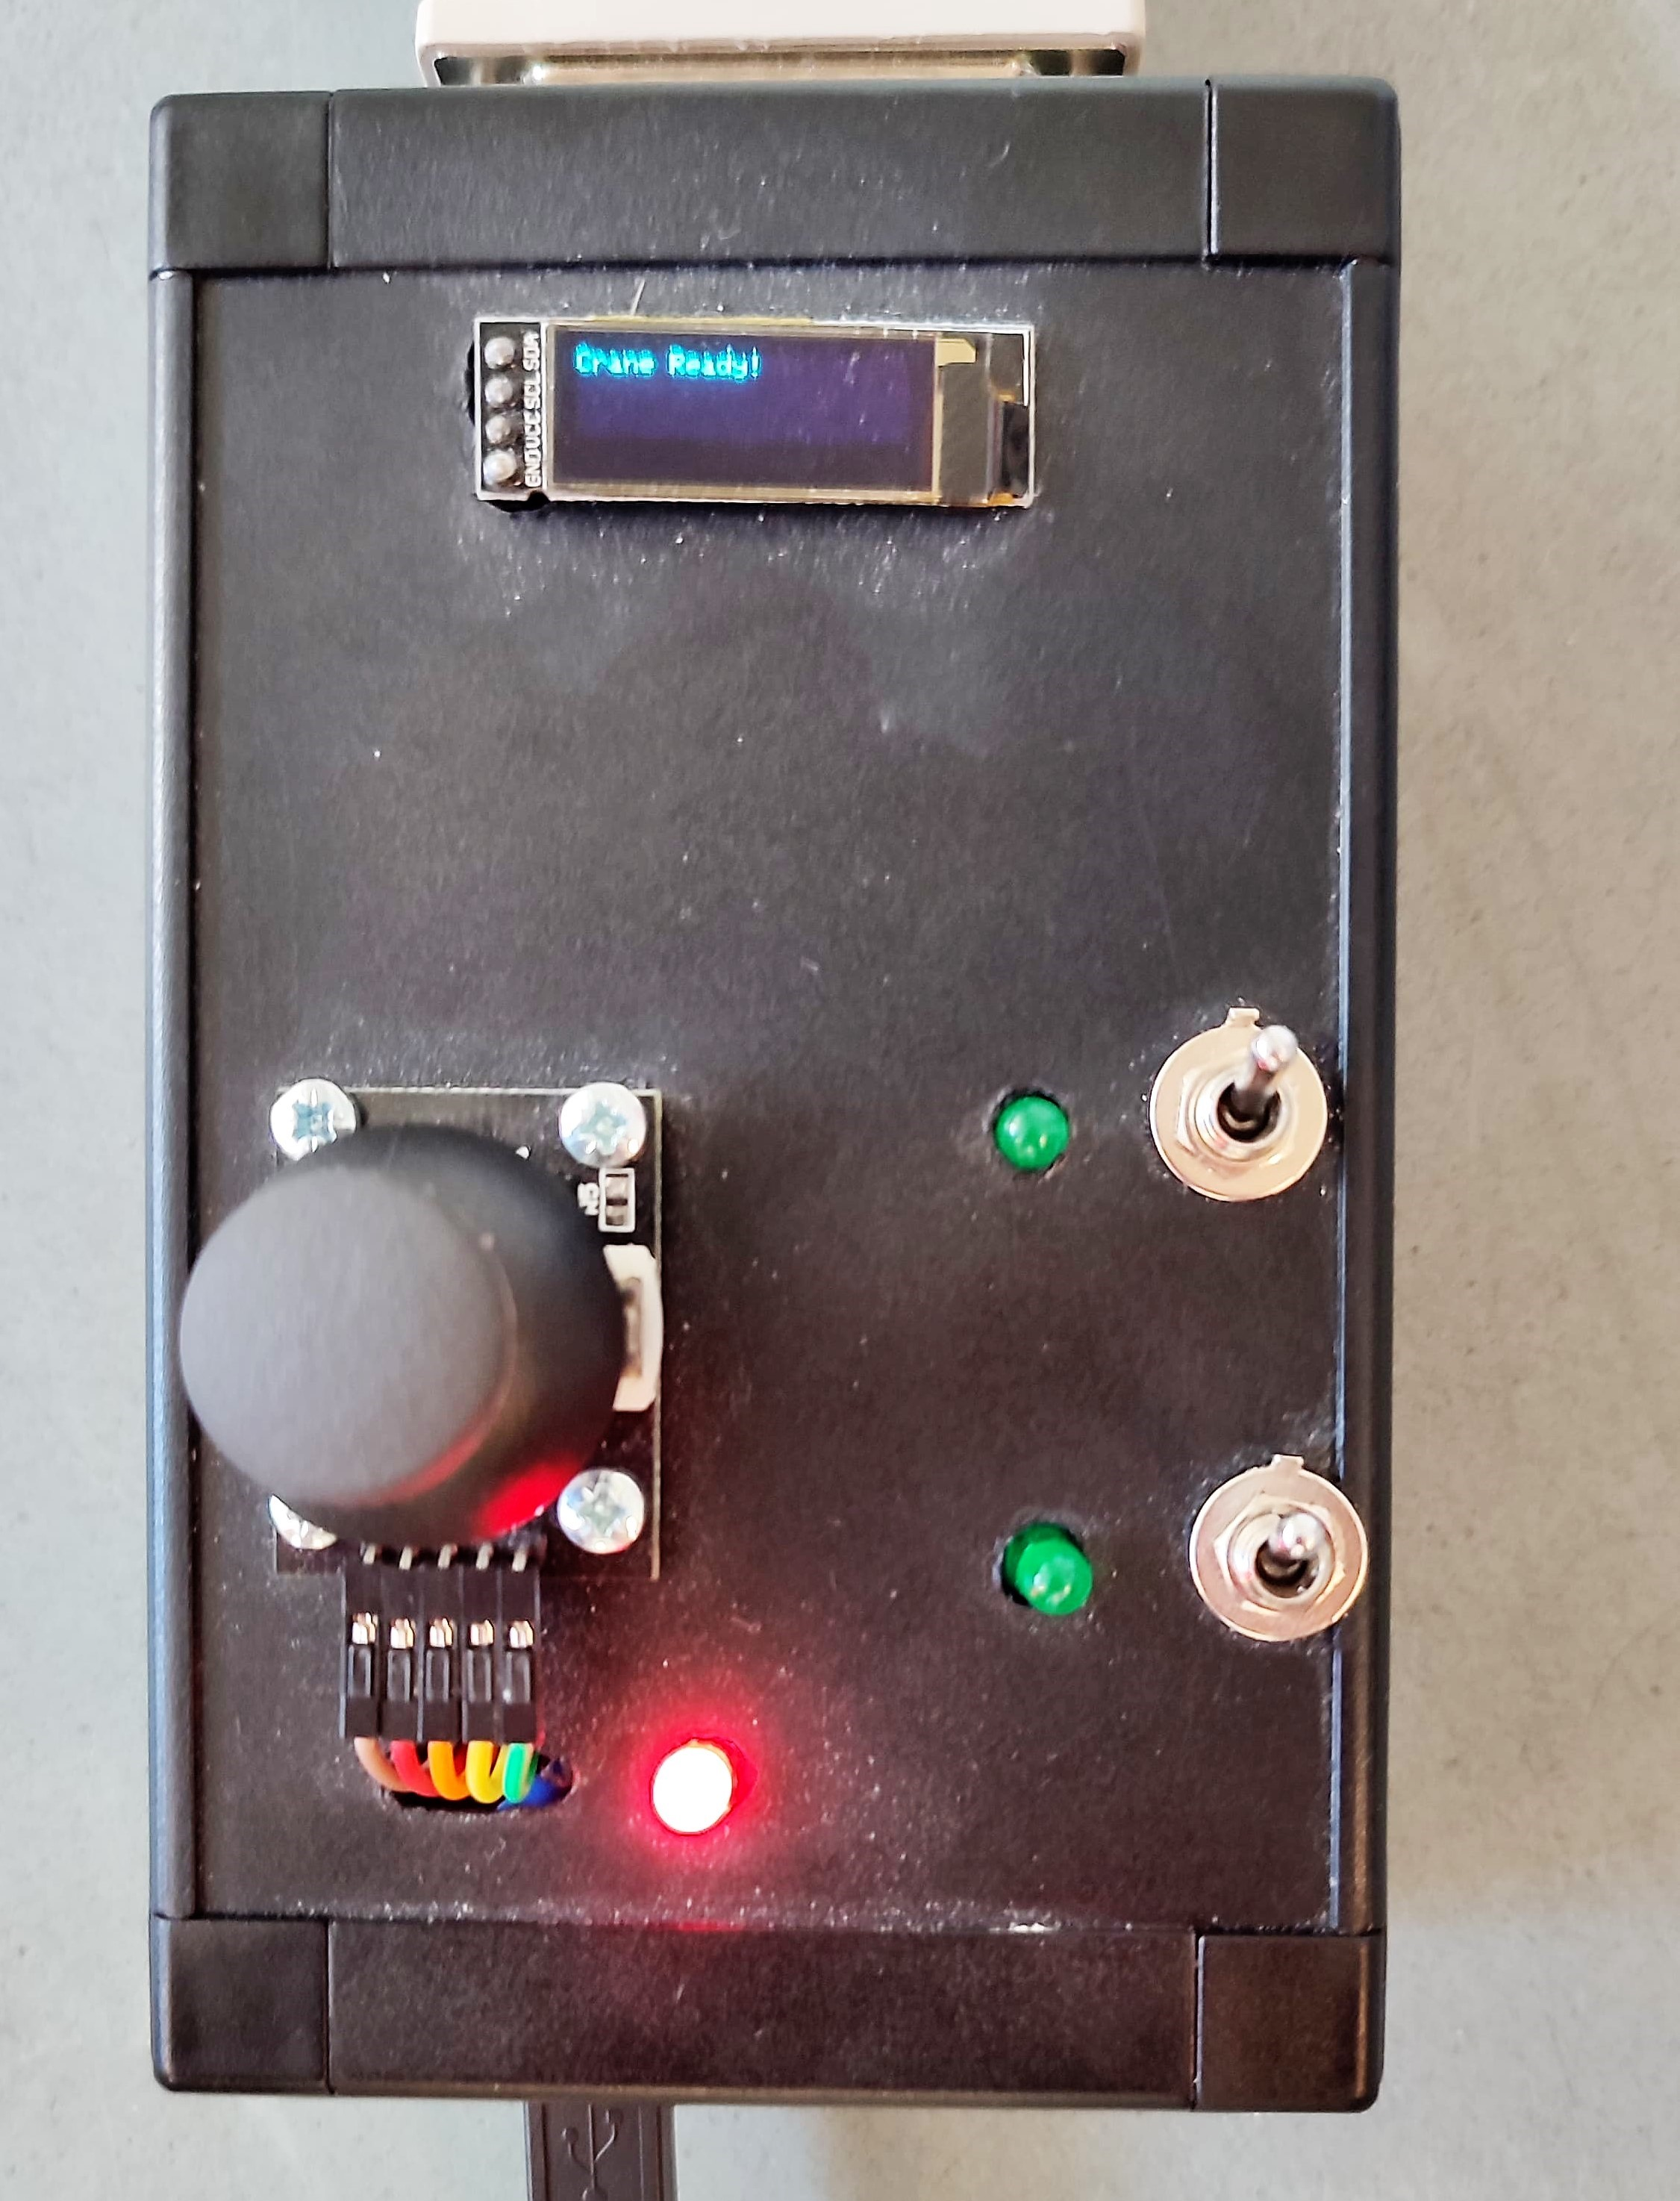
\includegraphics[width=0.4\textwidth]{pictures/manualController2Beskaaret.jpg}
    \caption{Controller layout.}
    \label{fig:pic_of_controller}
\end{figure}
\todo{add new picture with display}

The connections to the \amega are shown in figure \ref{fig:controller_connections}. All the pins without a connection on the \amega are unused and can be used to further expand the capabilities of the controller with more inputs and outputs. The L4941 located next to the display on figure \ref{fig:controller_connections} is a 5V regulator which ensures that the \amega internal voltage regulator does not get overloaded. The output of the L4941 is only used to power the display, but can also be used to power other \SI{5}{V} devices if needed.

%Tag fat i jakob, det er easyEDA fil, kan ikke dele den med link
\begin{figure}[H]
    \centering
    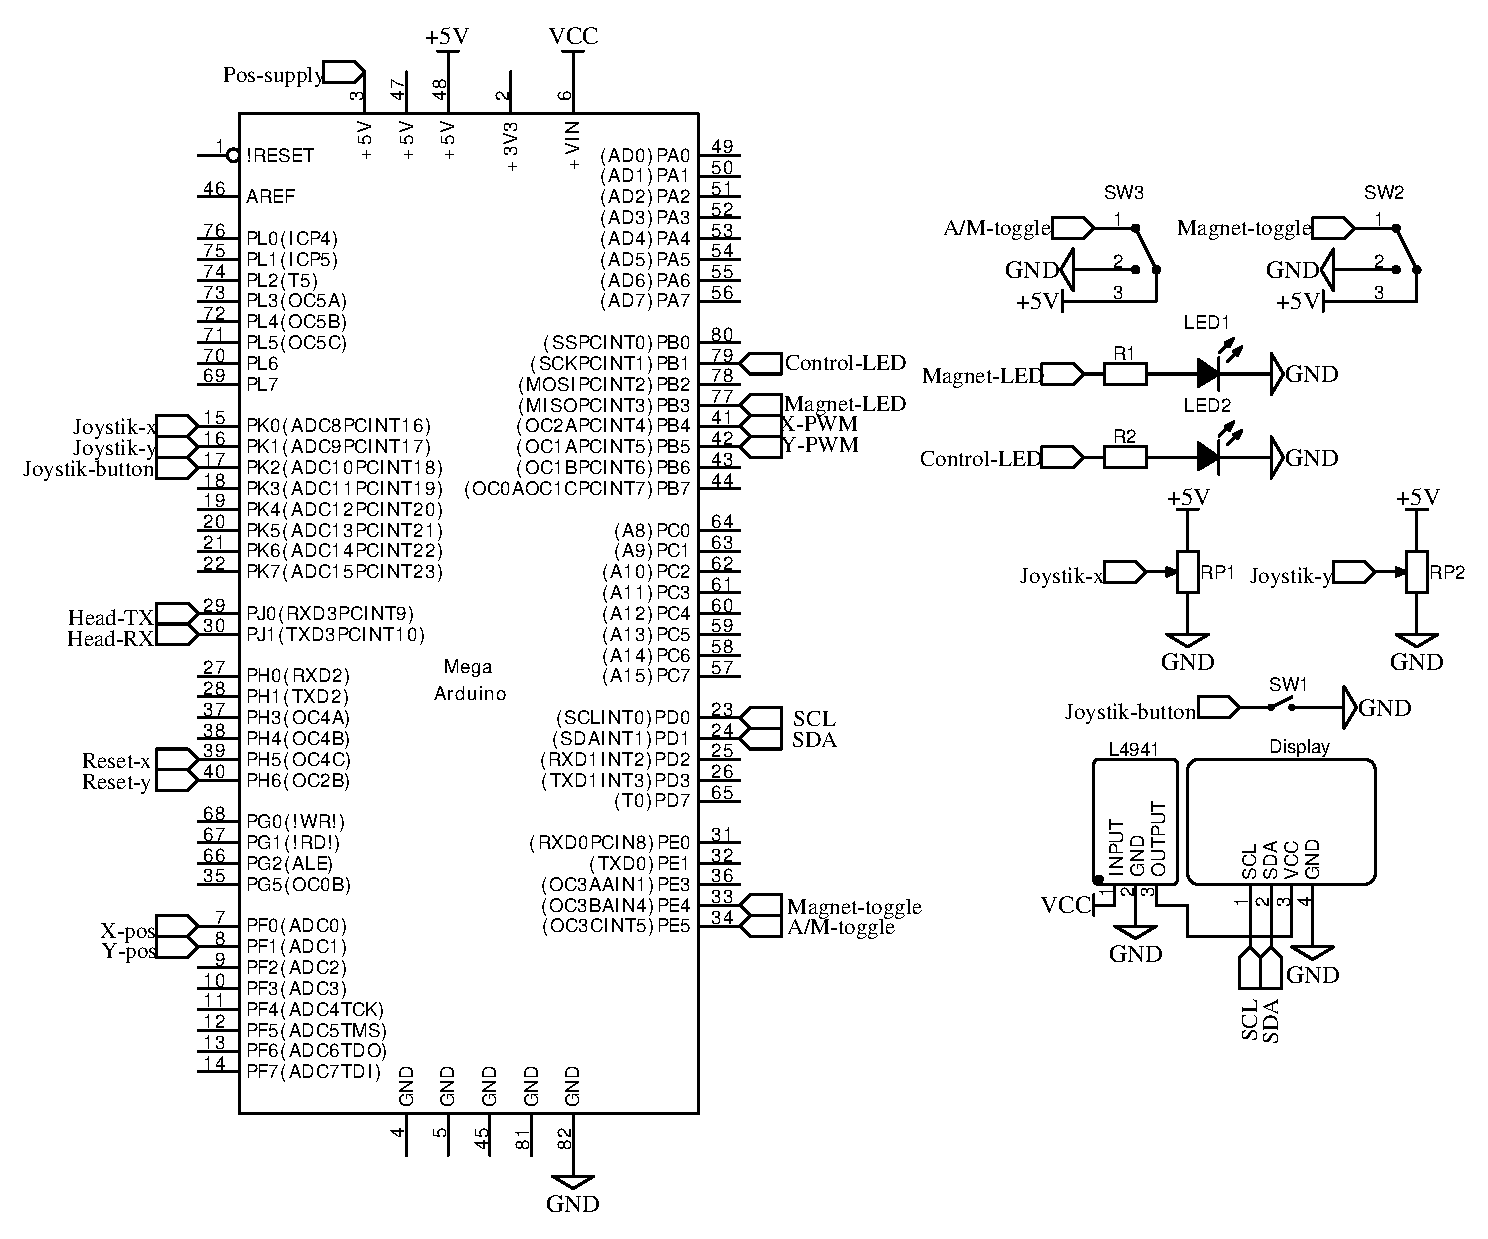
\includegraphics[width=1\textwidth]{pictures/Schematic_Kran_2022-02-16.pdf}
    \caption{Controller functional schematic.}
    \label{fig:controller_connections}
\end{figure}

\textbf{Links to hardware used:}\newline
L4941 \SI{5}{V} voltage regulator:\newline
\url{https://www.st.com/resource/en/datasheet/l4941.pdf}\\

Joystick:\newline
\url{https://www.amazon.com/SMAKN-Joystick-Breakout-Arduino-arduino/dp/B014MJLHC4}\\

\amega:\newline
\url{http://store.arduino.cc/products/arduino-mega-2560-rev3}\\

OLED screen:\newline
\url{https://dk.rs-online.com/web/p/oled-displays/2256197?cm_mmc=DK-PLA-DS3A-_-google-_-CSS_DK_DK_Displays_og_optoelektronik_Whoop-_-(DK:Whoop!)+OLED+displays-_-2256197&matchtype=&pla-302162021938&gclid=CjwKCAjw8sCRBhA6EiwA6_IF4cBCulk-WtMRrnzIQ23i7uNsbhB8FcUOVvLx726-mKff6_-QmLQVTRoCFzQQAvD_BwE&gclsrc=aw.ds}